% GNUPLOT: LaTeX picture with Postscript
\begingroup
  \makeatletter
  \providecommand\color[2][]{%
    \GenericError{(gnuplot) \space\space\space\@spaces}{%
      Package color not loaded in conjunction with
      terminal option `colourtext'%
    }{See the gnuplot documentation for explanation.%
    }{Either use 'blacktext' in gnuplot or load the package
      color.sty in LaTeX.}%
    \renewcommand\color[2][]{}%
  }%
  \providecommand\includegraphics[2][]{%
    \GenericError{(gnuplot) \space\space\space\@spaces}{%
      Package graphicx or graphics not loaded%
    }{See the gnuplot documentation for explanation.%
    }{The gnuplot epslatex terminal needs graphicx.sty or graphics.sty.}%
    \renewcommand\includegraphics[2][]{}%
  }%
  \providecommand\rotatebox[2]{#2}%
  \@ifundefined{ifGPcolor}{%
    \newif\ifGPcolor
    \GPcolortrue
  }{}%
  \@ifundefined{ifGPblacktext}{%
    \newif\ifGPblacktext
    \GPblacktextfalse
  }{}%
  % define a \g@addto@macro without @ in the name:
  \let\gplgaddtomacro\g@addto@macro
  % define empty templates for all commands taking text:
  \gdef\gplbacktext{}%
  \gdef\gplfronttext{}%
  \makeatother
  \ifGPblacktext
    % no textcolor at all
    \def\colorrgb#1{}%
    \def\colorgray#1{}%
  \else
    % gray or color?
    \ifGPcolor
      \def\colorrgb#1{\color[rgb]{#1}}%
      \def\colorgray#1{\color[gray]{#1}}%
      \expandafter\def\csname LTw\endcsname{\color{white}}%
      \expandafter\def\csname LTb\endcsname{\color{black}}%
      \expandafter\def\csname LTa\endcsname{\color{black}}%
      \expandafter\def\csname LT0\endcsname{\color[rgb]{1,0,0}}%
      \expandafter\def\csname LT1\endcsname{\color[rgb]{0,1,0}}%
      \expandafter\def\csname LT2\endcsname{\color[rgb]{0,0,1}}%
      \expandafter\def\csname LT3\endcsname{\color[rgb]{1,0,1}}%
      \expandafter\def\csname LT4\endcsname{\color[rgb]{0,1,1}}%
      \expandafter\def\csname LT5\endcsname{\color[rgb]{1,1,0}}%
      \expandafter\def\csname LT6\endcsname{\color[rgb]{0,0,0}}%
      \expandafter\def\csname LT7\endcsname{\color[rgb]{1,0.3,0}}%
      \expandafter\def\csname LT8\endcsname{\color[rgb]{0.5,0.5,0.5}}%
    \else
      % gray
      \def\colorrgb#1{\color{black}}%
      \def\colorgray#1{\color[gray]{#1}}%
      \expandafter\def\csname LTw\endcsname{\color{white}}%
      \expandafter\def\csname LTb\endcsname{\color{black}}%
      \expandafter\def\csname LTa\endcsname{\color{black}}%
      \expandafter\def\csname LT0\endcsname{\color{black}}%
      \expandafter\def\csname LT1\endcsname{\color{black}}%
      \expandafter\def\csname LT2\endcsname{\color{black}}%
      \expandafter\def\csname LT3\endcsname{\color{black}}%
      \expandafter\def\csname LT4\endcsname{\color{black}}%
      \expandafter\def\csname LT5\endcsname{\color{black}}%
      \expandafter\def\csname LT6\endcsname{\color{black}}%
      \expandafter\def\csname LT7\endcsname{\color{black}}%
      \expandafter\def\csname LT8\endcsname{\color{black}}%
    \fi
  \fi
    \setlength{\unitlength}{0.0500bp}%
    \ifx\gptboxheight\undefined%
      \newlength{\gptboxheight}%
      \newlength{\gptboxwidth}%
      \newsavebox{\gptboxtext}%
    \fi%
    \setlength{\fboxrule}{0.5pt}%
    \setlength{\fboxsep}{1pt}%
    \definecolor{tbcol}{rgb}{1,1,1}%
\begin{picture}(10080.00,5040.00)%
    \gplgaddtomacro\gplbacktext{%
      \csname LTb\endcsname%%
      \put(814,1540){\makebox(0,0)[r]{\strut{}$0$}}%
      \put(814,1895){\makebox(0,0)[r]{\strut{}$20$}}%
      \put(814,2250){\makebox(0,0)[r]{\strut{}$40$}}%
      \put(814,2605){\makebox(0,0)[r]{\strut{}$60$}}%
      \put(814,2960){\makebox(0,0)[r]{\strut{}$80$}}%
      \put(814,3314){\makebox(0,0)[r]{\strut{}$100$}}%
      \put(814,3669){\makebox(0,0)[r]{\strut{}$120$}}%
      \put(814,4024){\makebox(0,0)[r]{\strut{}$140$}}%
      \put(814,4379){\makebox(0,0)[r]{\strut{}$160$}}%
      \put(1437,1408){\rotatebox{-45}{\makebox(0,0)[l]{\strut{}Biometric Matching}}}%
      \put(1928,1408){\rotatebox{-45}{\makebox(0,0)[l]{\strut{}Convex Hull}}}%
      \put(2419,1408){\rotatebox{-45}{\makebox(0,0)[l]{\strut{}Count 102}}}%
      \put(2910,1408){\rotatebox{-45}{\makebox(0,0)[l]{\strut{}Count 10s}}}%
      \put(3401,1408){\rotatebox{-45}{\makebox(0,0)[l]{\strut{}Cryptonets (Max Pooling)}}}%
      \put(3892,1408){\rotatebox{-45}{\makebox(0,0)[l]{\strut{}Database Join}}}%
      \put(4383,1408){\rotatebox{-45}{\makebox(0,0)[l]{\strut{}Database Variance}}}%
      \put(4875,1408){\rotatebox{-45}{\makebox(0,0)[l]{\strut{}Histogram}}}%
      \put(5366,1408){\rotatebox{-45}{\makebox(0,0)[l]{\strut{}Inner Product}}}%
      \put(5857,1408){\rotatebox{-45}{\makebox(0,0)[l]{\strut{}k-means}}}%
      \put(6348,1408){\rotatebox{-45}{\makebox(0,0)[l]{\strut{}Longest 102}}}%
      \put(6839,1408){\rotatebox{-45}{\makebox(0,0)[l]{\strut{}Max. Dist. b/w Symbols}}}%
      \put(7330,1408){\rotatebox{-45}{\makebox(0,0)[l]{\strut{}Minimal Points}}}%
      \put(7821,1408){\rotatebox{-45}{\makebox(0,0)[l]{\strut{}MNIST ReLU}}}%
      \put(8312,1408){\rotatebox{-45}{\makebox(0,0)[l]{\strut{}Private Set Intersection}}}%
      \put(8935,1540){\makebox(0,0)[l]{\strut{}$0$}}%
      \put(8935,1824){\makebox(0,0)[l]{\strut{}$20$}}%
      \put(8935,2108){\makebox(0,0)[l]{\strut{}$40$}}%
      \put(8935,2392){\makebox(0,0)[l]{\strut{}$60$}}%
      \put(8935,2676){\makebox(0,0)[l]{\strut{}$80$}}%
      \put(8935,2960){\makebox(0,0)[l]{\strut{}$100$}}%
      \put(8935,3243){\makebox(0,0)[l]{\strut{}$120$}}%
      \put(8935,3527){\makebox(0,0)[l]{\strut{}$140$}}%
      \put(8935,3811){\makebox(0,0)[l]{\strut{}$160$}}%
      \put(8935,4095){\makebox(0,0)[l]{\strut{}$180$}}%
      \put(8935,4379){\makebox(0,0)[l]{\strut{}$200$}}%
    }%
    \gplgaddtomacro\gplfronttext{%
      \csname LTb\endcsname%%
      \put(209,2959){\rotatebox{-270}{\makebox(0,0){\strut{}Circuit Generation Time (sec)}}}%
      \put(9573,2959){\rotatebox{-270}{\makebox(0,0){\strut{}Improvement (number of times)}}}%
      \csname LTb\endcsname%%
      \put(2536,4867){\makebox(0,0)[r]{\strut{}GMW}}%
      \csname LTb\endcsname%%
      \put(2536,4647){\makebox(0,0)[r]{\strut{}GMW (Vectorized)}}%
      \csname LTb\endcsname%%
      \put(5503,4867){\makebox(0,0)[r]{\strut{}BMR}}%
      \csname LTb\endcsname%%
      \put(5503,4647){\makebox(0,0)[r]{\strut{}BMR (Vectorized)}}%
      \csname LTb\endcsname%%
      \put(8470,4867){\makebox(0,0)[r]{\strut{}GMW Improvement}}%
      \csname LTb\endcsname%%
      \put(8470,4647){\makebox(0,0)[r]{\strut{}BMR Improvement}}%
    }%
    \gplbacktext
    \put(0,0){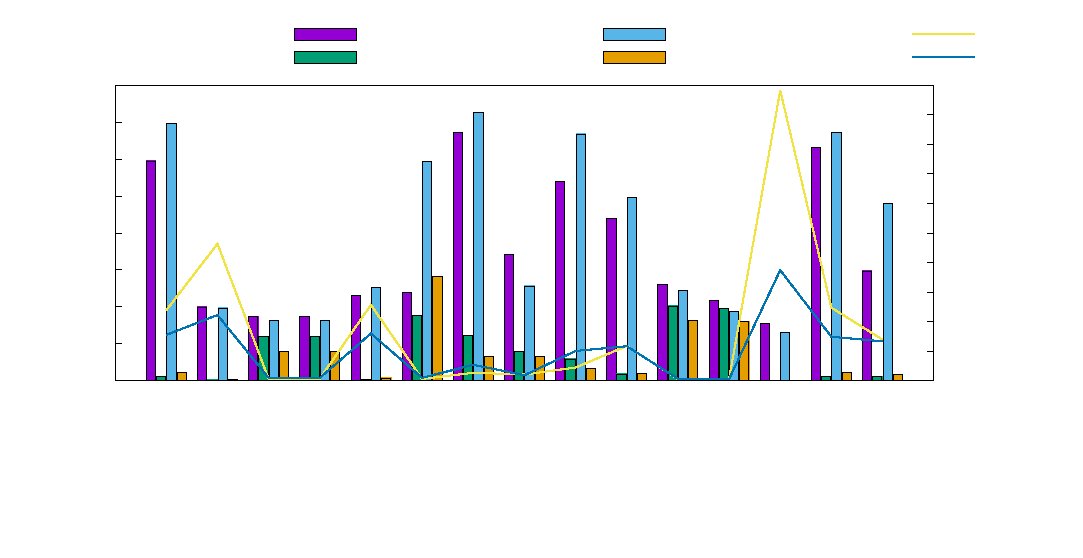
\includegraphics[width={504.00bp},height={252.00bp}]{all-hist-CircuitGenerationTimesec}}%
    \gplfronttext
  \end{picture}%
\endgroup
